\label{section:case-studies:vsmt}
%
\begin{figure}[h]
  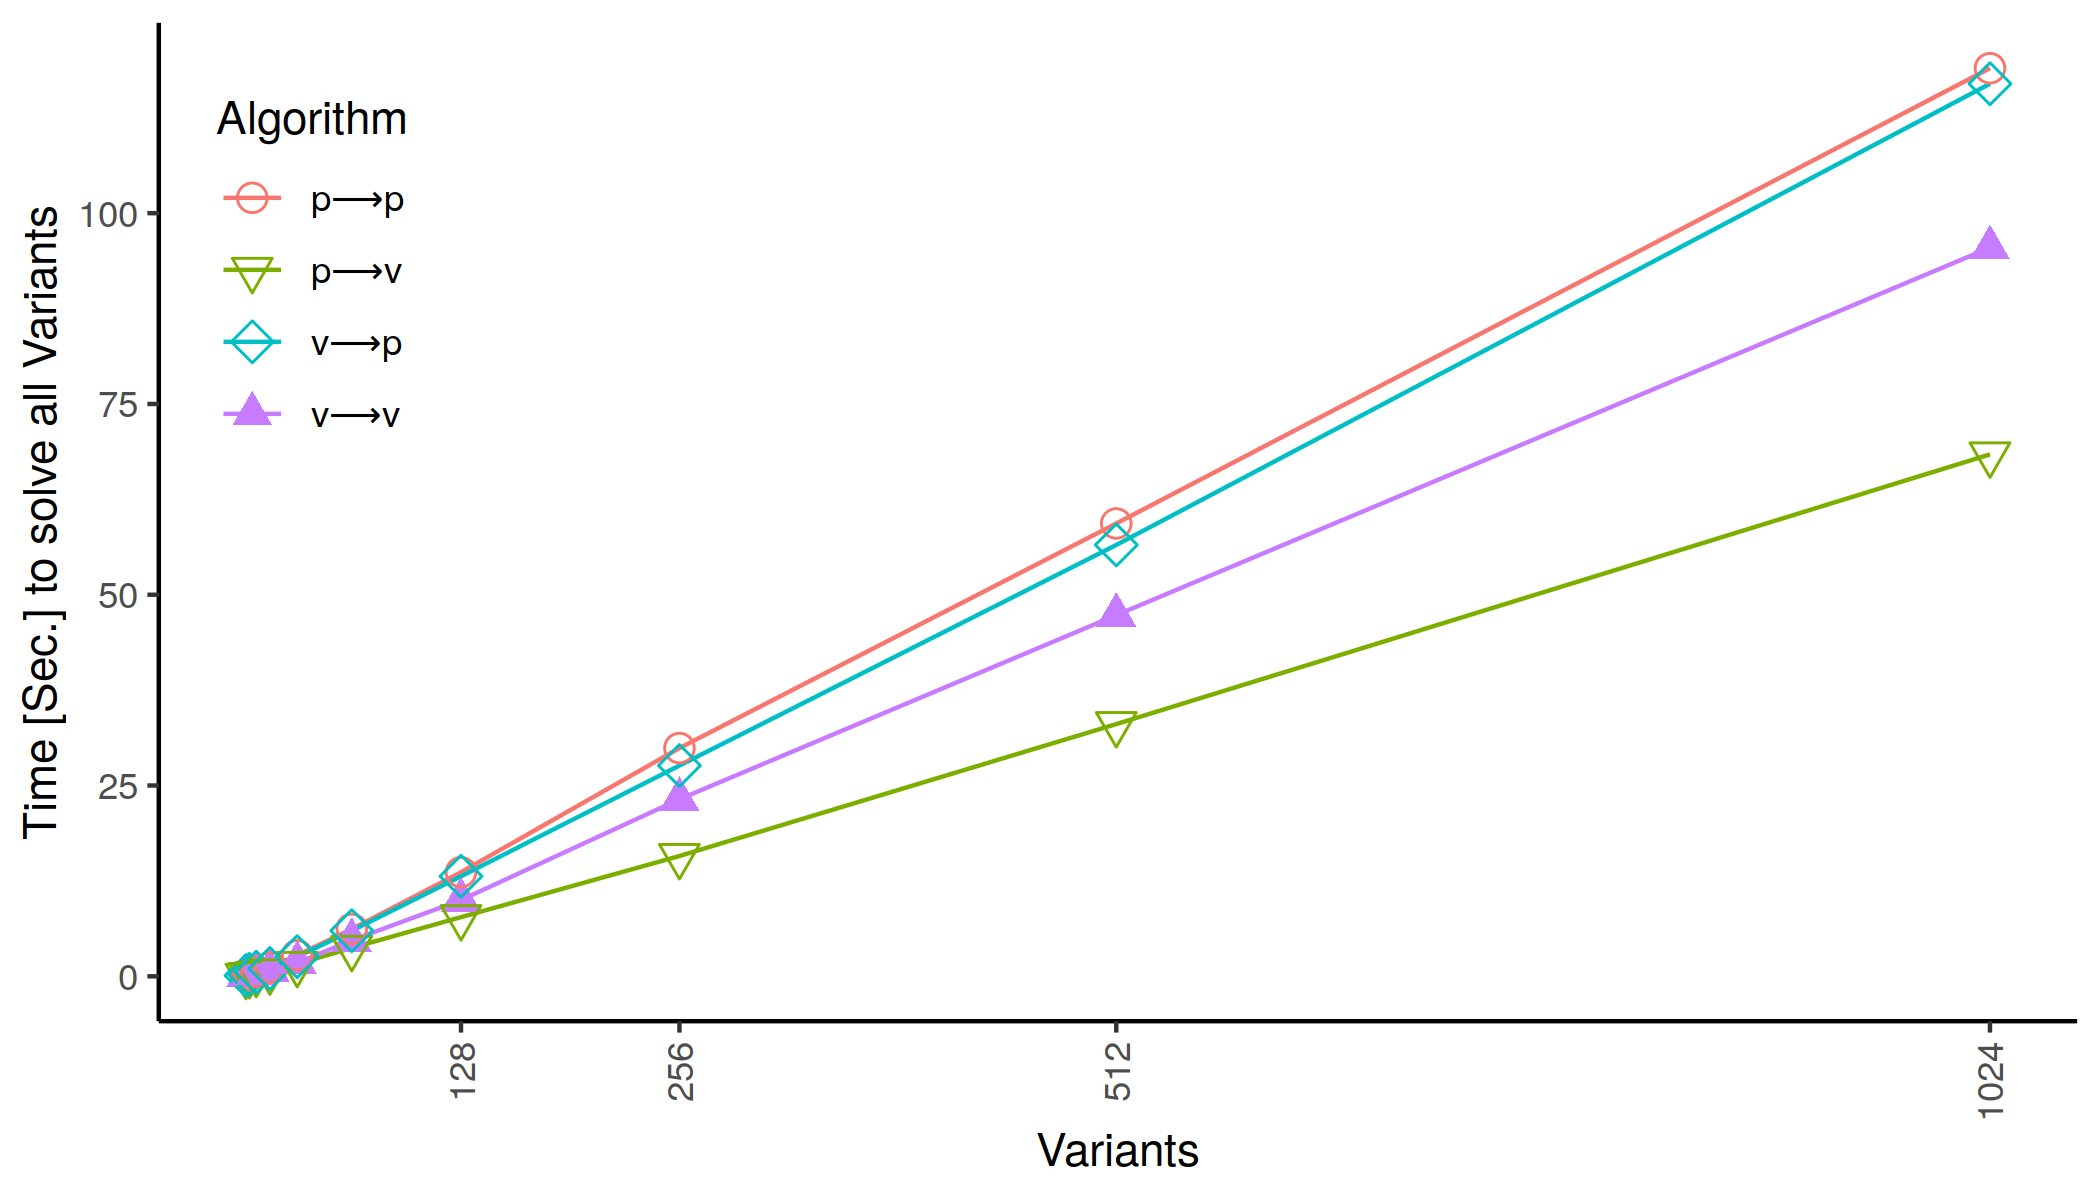
\includegraphics[width=0.95\textwidth]{Plots/RQ1_Fin_Smt}
  \caption{(Financial) Performance as variants increase for the variational
    \ac{smt} solver.}%
  \label{res:rq1:vsmt}
\end{figure}
%
We have shown that the variational \ac{sat} solver exhibits speedup for two
real-world datasets and that the sharing ration of a \ac{vpl} formula is a
significant factor in that speedup. However, we have yet to show that the same
is true for the prototype variational \ac{smt} solver, \vsmt{}.

To test \vsmt{} we use an \ac{smt} version of the \fin{} dataset from \nieke{}'s
study. Unfortunately, only the \fin{} dataset has an \ac{smt} version and so our
evaluation of the prototype \ac{smt} solver is limited. Furthermore, in the
course of encoding the dataset to a \evpl{} formula we discovered type errors in
1,514 formulas out of a total of 4,621 formulas. To utilize the dataset we
detected and corrected the type errors during parsing. Each error was identical
and revolved around the encoding of a \rn{one-of} constraint; where only one
constraint out of a sequence of constraints can be true. For example, an
incorrect version would be: $(f_{i} \equiv{} 1) \equiv{} (f_{0} + f_{1} \ldots{}
+ f_{n})$ for some $i$ and $n$. Thus, the error is that $f_{i} \equiv 1$ yields
a Boolean constraint (\ie{} $\equiv$ has type $\equiv{} : \eAR{} \rightarrow
\eAR{} \rightarrow{} \eIL{}$) but it is the left child of another $\equiv$ which
expects an arithmetic expression as its left child not a \eIL{} expression. The
correction is to repeat $f_{i}$ and handle the boolean constraint correctly. For
example the corrected version of the above formula is $(f_{i} \equiv{} 1)
\wedge{} (f_{i} \equiv{} (f_{0} + f_{1} \ldots{} + f_{n}))$, where we separate
out the left child from the summation but preserve the semantics of the
\rn{one-of} constraint.

\autoref{res:rq1:vsmt} displays the performance of \vsmt{} as variants to solve
increases. The resulting \evpl{} formula matched the number of choice and plain
terms from the \vsat{} version. Similarly, the number of satisfiable variants
matched the results for the \fin{} dataset in \autoref{res:vmodels}. \vsmt{}
displays a speedup of 1.22x over the baseline \vTop{} at 1,024 variants. There
are two significant differences between the \vsmt{} and \vsat{} results. First,
the prototype \ac{smt} solver \emph{does not} depend on the Haskell library
\texttt{sbv}. Instead, \vsmt{} utilizes a foreign-function interface to the C
API of z3. Consequently, where \texttt{sbv} utilizes strings over
\texttt{stdout} to communicate to the base solver, the ffi \vsmt{} uses utilizes
bytecode and hence has higher throughput. This has several implications, first,
the range of results \autoref{res:rq1:vsmt} are measured in seconds rather than
minutes such as \autoref{res:rq1:auto} and \autoref{res:rq1:fin}. Secondly, the
overhead case \pTov{} shows a speedup of 1.71x over the same baseline and is
consistently faster than the variational case \vTov{}. There are several
possible explanations but the exact reason is unclear.

We speculate on possible causes, \pTov{} computes the variant by
accumulation/evaluation, reducing the entire variant to a single symbolic and
then issuing a \rn{check-sat} call. Thus, any difference between \vTov{} and
\pTov{} must come from choice removal.
%
This is significant because this result may be a case where the extra work
induced by the evaluation context in choice removal does not yield performance
increases. To be specific, \vTov{} constructs a context to efficiently reuse
symbolic values, but if the \ac{smt} problem is very simple or if there exists a
tautology or contradiction that is plain, then \vTov{} will still construct and
operate on this context even each variant does not need to be computed. Thus, it
could be the case that for the majority of variants a contradiction or tautology
occurred and was found by z3 before the variation terms were considered (before
the \rn{push}/\rn{pop} calls) and thus any extra work to compute the result for
the variant was redundant.

The exact reason for this result is unclear and more data is required to
understand the prototype \ac{smt} implementation. Discovering the definitive
reason is left to future work. If an early tautology or contradiction is the
culprit then this could be detected in preliminary check. For example, one could
replace each choice in the variational core with \tru{} and issue a
\rn{check-sat} to check that the core is satisfiable before computing the
satisfiability of the variants. Similarly, it also could be the case that
particular sets \ac{smt} and \ac{sat} problems do not gain as much speedup from
variational solving. For example, they might trigger heuristics in the base
solver that simplify the problem space, and thus do not benefit from variational
solving. Detecting such sets would require more data to understand the
interaction between the variational \ac{sat} and \ac{smt} problems and the
variational solver. However, the overall result: that \vTov{} outperforms the
baseline case \vTop{}, is further demonstration that our methods are effective
for the three datasets we tested.

The last significant result is the magnitude of difference in the runtime
between the variational \ac{smt} prototype and variational \ac{sat} prototype.
Such a difference is to be expected given their implementation differences, but
this difference indicates \emph{other} domains where applying variation as a
computational concept might be useful. As we have shown (perhaps unsurprisingly)
performance benefits from using the concept of variation are greater when the
cost of a single transaction to the object language is high. This is the case
for the variational \ac{sat} solver, since the sbv library communicates to the
base solver process using strings. Thus in the prototype \ac{sat} solver, we
observe a greater performance speedup (3.51x) than we the cost is low, such as
in the prototype variational \ac{smt} solver (1.22x). This implies that other
domains where a transaction cost is high are likely to benefit from research on
variation. These domains might include network communication, where throughput
and response times can be significant, or file systems and databases, where disk
accesses are the limiting performance factor. In either case, this project
successfully demonstrates performance speedups for two real-world cases in
\ac{sat} and \ac{smt} solving by employing variational concepts.
